% Chapter 5 - Process Arrival Pattern Awareness

% \glsresetall % reset the glossary to expand acronyms again
\chapter[Process Arrival Pattern Aware Large Message GPU Allreduce]{Process Arrival Pattern Aware Large Message GPU Allreduce}\label{ch:CH5-PAPAwareness}
\index{Process Arrival Pattern Awareness}

\section{Motivation}
This chapter approaches allreduce collective design through the lens of \gls{PAP} awareness.
When designing collective algorithms, developers often assume that all processes arrive simultaneously, but this is not a safe assumption.
The order and timing that processes enter the collective can impact the algorithm's performance, and this work tries to leverage the arrival imbalance to improve the overall collective performance.
\gls{DL} is a challenging application to load balance due to the stochastic nature of datasets, leading to increased arrival imbalance at collectives \cite{Mohammadalizadehbakhtevari2021Thesis, Alizadeh2022PAPCollDL, Li2020DLPartialColl}. 
While \gls{PAP}-aware collective algorithms exist, no existing algorithms target multi-node \gls{GPU} deployments. 
To fill this gap, we propose a \gls{UCX}-\gls{RMA}-based \gls{PAP} distribution mechanism with an accompanying allreduce algorithm.
Our method performs better than existing \gls{SOTA} allreduce algorithm under imbalanced arrivals, and the performance improvements also translate to Horovod.

There are previously proposed methods and algorithms that leverage \gls{PAP} awareness to accelerate collectives, this chapter starts by surveying existing work.
We provide some analysis on how \gls{PAP} affects collectives and describe our approach to accelerating allreduce.
The main contribution is a novel cluster-wide method of sharing \gls{PAP} information with an accompanying allreduce algorithm designed to perform better than existing algorithms under a processes arrival imbalance.
We evaluate our work using an imbalance factor-inducing micro-benchmark, which can see a 60\% improvement over default \gls{MPI} implementations and 19\% over \gls{SOTA} algorithms.
We also use our method to evaluate Horovod throughput and see that synthetic benchmarks can improve 40\% over default and 7\% over \gls{SOTA}.

\subsection{Related Work}
Mamidala et al. \cite{Mamidala2004BarrierAllreduceIBAdaptive} propose a \gls{PAP}-Aware tree-based algorithm that can be applied to barrier and allreduce collectives.
Their method involves rebalancing a k-ary tree by passing a token between ranks.
For the process holding the token, when $k-1$ child processes have arrived, the token is passed to the $k^{th}$ child through an \gls{RDMA} write.
If an arriving process holds the token and all its child processes have arrived, it knows it is the last to arrive, so it triggers a multicast releasing all ranks from the barrier. 

Faraj et al. \cite{Faraj2008StudyProcArrivalMPIColl} evaluate process arrival imbalance at collectives across a handful of \gls{MPI} kernels.
The PMPI profiling interface was used to introspect the kernel runtime and collect \gls{PAP} statistics on two clusters.
The authors determine that process imbalance is unavoidable.
Even if the workload is perfectly balanced at the application level, the complexity of these massive systems will inevitably lead to differences in arrival time. 
However, regular imbalance patterns emerge during application runtime, and specific collective call sites will exhibit the same imbalance multiple times during execution.
They also measure the effect of process imbalance on specific algorithms for broadcast and alltoall outlining how process imbalance can be an important factor in algorithm selection.
The authors propose a method for \gls{PAP}-aware dynamic algorithm selection based on STAR-MPI \cite{Faraj2006StarMPI}.
This method monitors collective execution at the granularity of each call site and selects an optimal algorithm based on observed \gls{PAP} Imbalance. 

Patarsuk and Yuan \cite{Patarasuk2008EffBcastDifProcArr} investigate the impacts of \gls{PAP} on broadcast algorithms.
Through modelling, they show how all existing algorithms can suffer from substantial performance loss to process imbalance. 
The authors propose a new broadcast algorithm that dynamically assembles sub-groups to perform the broadcast operation.

Qian and Afsahi \cite{Qian2009ProcArrivalSHMA2AIB} propose a method for applying \gls{PAP}-Awareness to alltoall in InfiniBand Clusters.
They modify a direct alltoall algorithm so that data exchanges are not ordered.
The algorithm is built on top of InfiniBand's \gls{RDMA} semantics, meaning processes need to share destination addresses into which peers can write data. 
Their method relies on the \gls{RDMA} address as a notification mechanism alerting processes of when their peers arrived and where to write relevant data.
They also extend this idea to a hierarchical algorithm, allowing them to leverage shared memory for intranode transfers.

Parsons and Pai \cite{Parsons2015ExpProcImbMPICollHierarcialSys} study process imbalance on Cray XE6 using methods similar to Faraj et al. \cite{Faraj2008StudyProcArrivalMPIColl}.
They go a bit more in-depth by investigating performance counters using PAPI \cite{Mucci1999PAPI}. 
Still, they arrive at the same conclusion that the system is too complex and that none of the observable counters strongly correlate with processing imbalance. 
The authors propose a dynamic leader selection method to build hierarchical \gls{PAP}-aware algorithms for reduce and broadcast.
They use a shared memory structure for intranode communications, where the last/first processes to arrive are selected as the leader for the reduce/broadcast algorithms, respectively. 
Since any rank could be dynamically selected as a leader, parent/child relationships for the internode binomial tree are established using control messages with \texttt{MPI\_ANY\_SOURCE}. 
They also propose an alltoall algorithm, but they found that the overhead of the control messages is too significant, so instead, they impose a static multileader hierarchical pattern.
To take advantage of arrival patterns, the authors propose \textit{opportunistic message fragmentation}, criteria that leaders can use to select chunks of data to send before all processes have arrived.
This work only applies \gls{PAP} awareness at an intra-node level, their method does have a leader identification mechanism to set up inter-node exchanges, but it does not leverage any \gls{PAP} information.

Omer et al. \cite{Arap2015AdaptiveRDForCC} propose a method for decoupling the synchronization between rounds of a recursive doubling allreduce algorithm. 
This is accomplished by removing the strict ordering imposed through rounds of communication and instead managing messages through tag values.
The relaxed ordering can lead to duplicate reductions, so ranks are responsible for tracking which reduced results they have received and drop messages where appropriate. 
They evaluated their work on a NetFPGA platform \cite{Lockwood2007NetFPGA}, allowing them to fully offload their collective algorithm, and exploit network-level features like multicast, but limited their work to only use min/max operations.

Marendic et al. \cite{Marendic2016Clairvoyant} propose a \gls{PAP}-aware reduction algorithm.
Through theoretical analysis, they identify a lower bound for \gls{PAP}-Aware reduction, demonstrating that no matter the \gls{PAP}, any algorithm is bound by the times it takes for two processes to make a reduction, so they focus their efforts on doing that step as fast as possible. 
Their solution is a greedy algorithm to build a reduction schedule, but they have no method of detecting the \gls{PAP} and assume it is known beforehand.

Proficz published a series of algorithms for different collectives based on a process arrival estimation method \cite{Proficz2018ImprvAllReduceForImbPAP, Proficz2020PAPAwareScatterGather, Proficz2021AllGatherResilientToImbPAP}.
Their method targets bulk-synchronous parallel applications with distinct computation and communication phases.
To estimate a process's arrival time, application developers embed a callback to notify a background process when the computation phase is almost complete.
This background thread uses this information to reorder processes in a collective algorithm to make more optimal use of arrival imbalance.
The author proposes methods for reordering direct, ring, and binomial algorithms to accelerate, allreduce, scatter, gather and allgather collectives.

Alizadeh et al. \cite{Alizadeh2022PAPCollDL} presented a series of ideas for handling \gls{PAP} in collectives. 
The author proposed two methods, targeting small and large messages, for handling arrival synchronization and message exchanges within a node.
The proposed work relies on incrementing a shared memory counter and writing data into appropriate buffers.
Their method only detects \gls{PAP} at an intranode level, but they evaluate the efficacy of extending to a hierarchical algorithm to handle cluster-wide collectives.

\section{Design Methodology}
\subsection{PAP Arbitration Mechanims}
For ranks to determine the arrival order, we took inspiration from the small message synchronization method used by Alizadeh et al. \cite{Alizadeh2022PAPCollDL} and extended it to a multi-node setting.
Synchronization depends on a data structure consisting of a counter for arrival position and an array for arrival-to-rank translations, an outline of the structure and how it is used is provided in Figure \ref{fig:fig_sync_structur}.
In order to target a distributed memory environment, the data structure resides in network-exposed memory on a predetermined process and is accessed through one-sided network operations.
When a process arrives at the collective, it fetch-and-increments the counter to determine its arrival position and then writes its rank into the arrival array indexed at its arrival position.
Accessing the counter creates a critical section, potentially adding overhead if not accounted for.
When a process arrives, it can determine which ranks have arrived before it by indexing their arrival position in the arrival-to-rank translation array.
For simplicity, we use a contiguous buffer allocated next to the arrival counter.
A more complicated design could distribute the arrival array so that each process exposes a subset of indexes, this would more evenly distribute both memory requirements and network resource demand.

% This imposes a memory requirement that scales linearly with the number of processes.
% We did not run into scaling issues with the system we used for evaluation, but larger systems that can run jobs on the order of millions of .
% Further, a more complicated design could distribute the arrival array so that each process exposes one index, more evenly distributing both memory requirements and network resource demand.

\begin{figure}
    \centering
    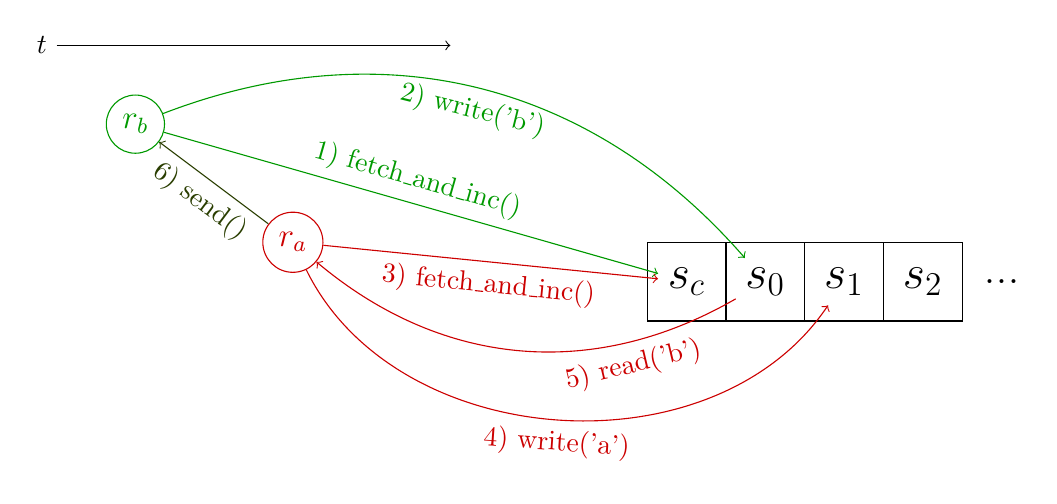
\begin{tikzpicture}[
        nsty/.style={circle,draw,font=\large},
        ssty/.style={font=\LARGE},
        ]
    
        \node (sc) at (1,0) [ssty] {$s_c$};
        \node (s0) at (2,0) [ssty] {$s_0$};
        \node (s1) at (3,0) [ssty] {$s_1$};
        \node (s2) at (4,0) [ssty] {$s_2$};
        \node (scont) at (5,0) [ssty] {...};
        
        \node (ra) at (-4,0.5) [nsty,color=red!80!black] {$r_a$};
        \node (rb) at (-6,2) [nsty,color=green!60!black] {$r_b$};
    
        \draw[->]  (-7,3) node[left] {$t$} --  (-2,3);
    
        \draw (0.5,-0.5) rectangle (1.5,0.5);
        \draw (1.5,-0.5) rectangle (2.5,0.5);
        \draw (2.5,-0.5) rectangle (3.5,0.5);
        \draw (3.5,-0.5) rectangle (4.5,0.5);
    
        \draw[->,color=green!60!black] (rb) -- node[above,sloped,color=green!60!black] {1) fetch\_and\_inc()} (sc);
        \draw[->,color=green!60!black] (rb) to [bend left=35] node[below,sloped,color=green!60!black] {2) write('b')} (s0);
        \draw[->,color=red!80!black] (ra) -- node[below,sloped,color=red!80!black] {3) fetch\_and\_inc()} (sc);
        \draw[->,color=red!80!black] (ra) to [bend right=60] node[below,sloped,color=red!80!black] {4) write('a')} (s1);
        \draw[->,color=red!80!black] (s0) to [bend left=35] node[below,sloped,near start,color=red!80!black] {5) read('b')} (ra);
        \draw[->,color=red!40!green!40!black] (ra) to node[sloped,below] {6) send()} (rb);
        
    \end{tikzpicture}
    \caption[Proposed Process Arrival Pattern Distribution Mechanism]{
        Depiction of arrival discovery mechanism.
        $r_b$ arrives first, fetch-and-increments the counter, and writes it's rank into index $s_0$.
        $r_a$ arrives after, fetch-and-incremens the counter and claims $s_1$. 
        After $r_a$ arrives, it can read the ranks of earlier arrivals to send them data if necessary.
    }
    \label{fig:fig_sync_structur}
\end{figure}


% \subsection{Arrival Syncronization}
In terms of implementation, we want to leverage a higher-level programming interface for portability, and our first choice would be \gls{MPI}'s one-sided communications, but the problem with \gls{MPI} is that the message completion and synchronization model is too burdensome. 
The counter can be incremented through \texttt{MPI\_Fetch\_and\_op()}, but atomicity and completion must be enforced through a synchronization mechanism. 
Active target communication is out of the question as one of our goals is to minimize the amount of synchronization, and \texttt{MPI\_Win\_Fence()} is a collective, so it also defeats the purpose.
This leaves \texttt{MPI\_Win\_lock()}/\texttt{MPI\_Win\_unlock()} as the only viable synchronization mechanism.
Alternatively, we could go deeper down the stack and use a transport layer API since they provide the desired portability with an acceptable performance penalty.
Specifically, we use \gls{UCX}'s \gls{RMA} and atomic operations \cite{shamis2015ucx}.
\texttt{ucp\_atomic\_op\_nbx()} is specified to be atomic with respect to all other \gls{UCX} operations allowing us to increment the counter variable atomically, and operation completion is guaranteed on a per-message level, removing the requirements for the heavy barrier-like synchronization \gls{MPI} enforces.

In deciding to use \gls{UCX} over \gls{MPI}, we wrote a benchmark to evaluate the overhead of one-sided operations and synchronization, the structure of which is provided in Algorithm \ref{alg:sync_struct_bmark}.
The core of the benchmark is evaluating how long it takes to atomically increment a memory location (Line 7) and perform a write to a separate location (Line 9), analogous to the \gls{PAP} arbitration mechanism.
The fetch-and-add needs to complete before the write can be issued, so appropriate completion mechanisms must be used (Line 8).
The most performance-critical parts of the benchmarks would be the remote synchronization calls (Lines 8 and 10), this is where the differences between \gls{MPI} and \gls{UCX} are apparent.  

\begin{algorithm}
  \caption{Generic sturcture of syncronization structure benchmark}
  \label{alg:sync_struct_bmark}
  \begin{algorithmic}[1]
    \Require Number of itterations $n$, Number of warmups $w$, communicator $comm$, remote memory $m$
    \Ensure The cost of syncronization $t$
    
    \State $t\_sum =$ 0
    \For{ $i$ in 0 to $w + i$}
        \If{mpi rank is 0}
            \State reset\_remote\_memory($m$)\Comment{prepare $m$ for syncronization}
        \EndIf
        \State MPI\_Barrier($comm$)
        \State $t\_start =$ MPI\_Wtime()
        \State remote\_fetch\_and\_add(\&$m[0]$, 1, \&$fadd\_val$)\Comment{Atomicly incremet remote value}
        \State wait\_preverous\_remote\_mem\_op()\Comment{Ensure memory operation completes}
        \State remote\_write(\&$m[fadd\_val+1]$, $rand\_val$)\Comment{Write to buffer based on f}
        \State wait\_preverous\_remote\_mem\_op()\Comment{Ensure remote memory operation completes}
        \State $t\_sum += (i-w >= 0)$ ? 0 : MPI\_wtime() - $t\_start$\Comment{save timings if not doing a warmup run}
    \EndFor
    \State MPI\_Reduce($t\_sum$, MPI\_SUM, 0) \Comment{Reduce measure runtimes to rank 0}
    \State $t = (t\_sum/n)/comm\_size$ \Comment{Return the measured time devided by the world size and the number of itterations}
  \end{algorithmic}
\end{algorithm}

We built two implementations of this benchmark, one with \gls{MPI} and the other with \gls{UCX}. 
To ensure memory completion in \gls{MPI}, we open and close an access epoch through calls to \texttt{MPI\_Win\_lock()}/\texttt{MPI\_Win\_unlock()} before and after each remote memory call.
On the other hand, completion in \gls{UCX} is guaranteed at a per-operation level. 
Every communication call returns a pointer to a structure which indicates the status of the operation, and at some point in the future (during a call to \texttt{ucp\_progress()}), the \gls{UCX} runtime will trigger a callback which modifies the pointer to indicate completion.
So to wait for remote memory completion, the \gls{UCX} benchmark polls the pointer while calling \texttt{ucp\_progress()} until completion.

We ran our benchmark on Narval, a 200G HDR InfiniBand cluster, using 32 nodes and scaling from 1 to 32 processes per node, and the results are presented in Figure \ref{fig:sync_bmark_32n}.
As is evident, the synchronization with \gls{MPI} has much more overhead than \gls{UCX}.
The benchmark time of \gls{UCX} scales linearly with the number of processes from 10$\mu s$ for 32 processes to 400$\mu s$ for 1024.
\gls{MPI} has more overhead, as with 32 processes, it takes 312$\mu s$, while it might also scale linearly, the largest runs are still an order of magnitude slower than \gls{UCX} at 453737$\mu s$ with 1024 processes.
Therefore, we decided to use \gls{UCX} to build our \gls{PAP} management mechanism, as \gls{UCX} provides wrappers around the necessary \gls{RDMA} and atomic network operations, there is no enforced synchronization model, and there are strong guarantees on operation completion. 

\begin{figure}
    \centering
    \begin{tikzpicture}
        \begin{semilogxaxis}[
        % \begin{loglogaxis}[
            title={Syncronization Method Comparison},
            xlabel={Number of Processes},
            ylabel={Sync time ($\mu s$)},
            legend entries={MPI, UCX},
            legend style={anchor=north, at={(0.5, -0.3)}},
            legend columns=2,
            xticklabels={32, 64, 128, 256, 512, 1024},
            xtick={32, 64, 128, 256, 512, 1024},
            % nodes near coords,
        ]
        \addplot table[x=ranks, y=mpirma] {3_Chapters/5_Chapter_PAPAwareness/Figs/bk_eval_ss_32n.dat};
        \addplot table[x=ranks, y=ucp] {3_Chapters/5_Chapter_PAPAwareness/Figs/bk_eval_ss_32n.dat};
        \end{semilogxaxis}
        % \end{loglogaxis}
    \end{tikzpicture}
    \caption{Comparison of rma syncronization methods with 32 nodes on Narval.}
    \label{fig:sync_bmark_32n}
\end{figure}

\subsection{PAP-Aware Hierarchical Chain Allreduce Algorithm}

In designing an algorithm, we aim to minimize the time the last arriving process needs to take.
For a ring or \gls{RSA} collective, when the last process arrives, it must send all messages in the algorithm.
Therefore, the last process in our collective algorithm must be able to complete its work with a bandwidth term smaller than $2n(\beta+\gamma)$. 
We can simplify the problem and look at a two-process allreduce, where the minimum amount of work involves receiving a message, performing a local reduction and sending a message, i.e., $2(\alpha+n\beta)+n\gamma$ \cite{Marendic2016Clairvoyant}.
We can remove the initial receive by sending the data ahead of time to a preallocated buffer, and the final send will need to become a broadcast, $n\gamma+T_{bcast}(n)$. 
If we use a pipelined chain broadcast algorithm, the last process only needs to reduce and send one message divided across $k$ segments, lowering the time to $T_{last\_proc\_reduce}=k\alpha+n(\beta+\gamma)$.
Every other process sends and receives $k$ messages of totalling $n$ bytes, given them a broadcast time of $k\alpha+n\beta$.
This is roughly half of the ring and \gls{RSA} bandwidth requirements for large messages.

A detailed outline of the proposed method is given in Algorithm \ref{alg:heir_pipe_chain}.
We embed our method in a hierarchical algorithm, this adds some implicit topology awareness and improves scalability.
The algorithm starts with an intranode reduction to a local leader process (Line 1), then the leader processes perform the \gls{PAP}-aware inter-node reduce (Lines 2-17), and the data is redistributed through internode and intranode broadcasts (Lines 18-27).
To improve pipeline efficiency, we overlap the internode broadcast and intranode broadcasts, which improves efficiency by overlapping the two stages of communication.

\begin{algorithm}
    \caption{PAP-Aware Pieplined Hierarchical Chain Allreduce}
    \label{alg:heir_pipe_chain}
    \DontPrintSemicolon
    % \KwIn{$buf$ - the buffer to perform an in-place allreduce on, $size$ - size of buffer, $seg\_size$ - segment size of pipeline, $intra\_comm$ - \texttt{MPI\_Communicator} for within the node, $inter\_comm$ - \texttt{MPI\_Communicator} for across nodes}
    % \KwIn{$buf$ - the buffer to perform an in-place allreduce on, $size$ - the size of $buf$, $intra\_comm$ - \texttt{MPI\_Communicator} for within the node, $inter\_comm$ - \texttt{MPI\_Communicator} for across nodes}
    \KwIn{A buffer of data with a datatype and size, an \texttt{MPI\_OP} to apply, a segment size for pipelining, and intra- and inter-node communicators.}
    \KwOut{An allreduce is performed in place on buf or on a specified output buffer.}
   \SetKwFunction{MPIReduce}{MPI\_Reduce}
   \SetKwFunction{MPIReducelocal}{MPI\_Reduce\_local}
   \SetKwFunction{MPIBcast}{MPI\_Bcast}
   \SetKwFunction{MPIIbcast}{MPI\_Ibcast}
   \SetKwFunction{MPICommrank}{MPI\_Comm\_rank}
   \SetKwFunction{MPICommsize}{MPI\_Comm\_size}
   \SetKwFunction{MPIIrecv}{MPI\_Irecv}
   \SetKwFunction{MPIRecv}{MPI\_Recv}
   \SetKwFunction{MPISend}{MPI\_Send}
   \SetKwFunction{MPIWait}{MPI\_Wait}
   \SetKwFunction{MPIWaitall}{MPI\_Waitall}
   
   % \MPIReduce{buf, size, 0, intra\_comm} \;
   Perform intra-node \MPIReduce{} \;

   \If{rank is leader of node}{
       $arrival$ = get\_arrival() \;
       
       \If{not the first to arrive}{
            $parent\_rank$ = get\_previous\_arrival() \;
       }
       
       \If{the first to arrive}{
            Receive $child\_rank$ from \texttt{MPI\_ANY\_SOURCE} and send data\; 
            % \MPIRecv{\&child\_rank, MPI\_ANY\_SOURCE} \;
            % \MPISend{buf, child\_rank} \;
       }\ElseIf{the second-last to arrive}{
            Inform $parent\_rank$ of arrival, receive data from $parent\_rank$ and perform local reduction \;
            Calculate $child\_rank$ based on processes that have already arrived \; 
            Send data to pre-posted buffer on $child\_rank$ \;
            % \MPIRecv{\&tmp\_buf, MPI\_ANY\_SOURCE} \;
            % \MPIReducelocal{buf, tmp\_buf} \;
            % $child\_rank$ = calc\_child\_rank() \;
            % \MPISend{buf, child\_rank} \;
       }\ElseIf{the last to arive}{
            Ensure the pre-posted buffer has data and perform local reduction \;
            Re-issue pre-posted buffer;
            % \MPIWait{pre\_posted\_req} \;
            % \MPIReducelocal{buf, pre\_posted\_buf} \;
            % \MPIIrecv{pre\_posted\_buf, MPI\_ANY\_SOURCE, \&pre\_posted\_req} \;
       }\Else{
            Inform $parent\_rank$ of arrival, receive data from $parent\_rank$ and perform local reduction \;
            Receive $child\_rank$ from \texttt{MPI\_ANY\_SOURCE} and send data\; 
            % \MPIRecv{\&tmp\_buf, MPI\_ANY\_SOURCE} \;
            % \MPIReducelocal{buf, tmp\_buf} \;
            % \MPIRecv{\&child\_rank, MPI\_ANY\_SOURCE} \;
            % \MPISend{buf, child\_rank} \;
       }

        $last\_arrival$ = get\_last\_arrival() \;
        
        % \MPIIbcast{buf, seg\_size, last\_arrival, inter\_comm, \&pipe\_bc\_req[0]} \;
        Issue first inter-node \MPIIbcast from $last\_arrival$ \;
        \For{ The number of segments minus 1 }{
            Wait for the previous iteration of \MPIIbcast to complete \;
            Issue inter- and intra-node \MPIIbcast on the appropriate segments \;
            % \MPIWaitall{pipe\_bc\_req} \;
            % \MPIIbcast{buf+$seg\_size * (i+1)$, seg\_size, last\_arrival, inter\_comm, \&pipe\_bc\_req[0]} \;
            % \MPIIbcast{buf+$seg\_size * i$, seg\_size, 0, intra\_comm, \&pipe\_bc\_req[1]} \;
        }
        Wait for the last inter-node \MPIIbcast to complete \;
        Start the last intra-node \MPIIbcast and complete any outstanding requests \;
        % \MPIWaitall{pipe\_bc\_req} \;
        % \MPIIbcast{buf+$seg\_size * (num\_segments -1)$, seg\_size, 0, intra\_comm, \&pipe\_bc\_req[1]} \;
        % \MPIWait{pipe\_bc\_req[1]} \;
    }\Else{
        \For{Each segment in the buffer}{
            Issue and complete intra-node \MPIIbcast for each pipeline segment \;
           %  \MPIIbcast{$buf+(seg\_size*i)$, seg\_size, 0, intra\_comm, \&intra\_bc\_req} \;
           % \MPIWait{intra\_bc\_req}
        }
   }
   % }
    % \MPIBcast{buf, 0, intra\_comm} \;
\end{algorithm}

We use a chain reduce to propagate the data to the last process. 
Each process receives a message from the previous arrival (its \textit{parent\_rank}), performs a local reduction, and forwards the result to the following arriving processes (its \textit{child\_rank}).
We chose a chain for its simplicity, however, it is not a scalable algorithm since both $\alpha$ and $\beta$ linearly correlate with $n$.
However, the bulk of our performance gains is derived from minimizing work at the last process. 
So even if the chain reduce takes a long time, as long as the last rank receives its data before it arrives (Line 11 completes before line 13), we should see performance improvements.

One issue is that \gls{MPI} ranks must know the destination before sending their data, and ranks that arrive early will not know the next rank until they arrive.
Our solution requires the \textit{child\_rank} to notify its \textit{parent\_rank} when it arrives with a small message.
While this does create a little overhead, it is negligible compared to large message transfer time.
The exception to this rule is the second to last rank, which can calculate its \textit{child\_rank} by finding the missing rank in the arrival-to-rank translation table (Line 10).
Once the \textit{child\_rank} is determined, the second last rank can forward its data ahead of time to a preposted \texttt{MPI\_Irecv} buffer (Line 11).
This lets the last rank quickly perform its local reduction and start broadcasting the result back to the other processes.

We use a chain algorithm for the internode broadcast and a knomial broadcast for intranode. 
We evaluated several broadcast algorithms with micro-benchmarks, including binary tree and scatter-allgather, and chose the above algorithms due to their performance.  
Pipelining is important as it lets us overlap the internode broadcast with the intranode broadcast improving latency.
By changing the segment size we can tune the algorithm to optimize performance.
If the segment size is larger than the message size, it is essentially 'turns of' pipelining, since there is only one pipeline segment, the algorithm collapses into two broadcasts.
This can be ideal in some scenarios, as pipelining can increase software overhead if the segment size is too small.

\section{Experimental Evaluation and Analysis}
\subsection{Experimental Platform}
We evaluated our proposed methods with a micro-benchmark and a synthetic Horovod benchmark on two clusters, Beluga and Narval.
We only focus on the \gls{GPU} resources this time.
Beluga's architecture is defined in Section \ref{sec:CH4-experimental-platform}.
Narval is very similar to Beluga but is made up of newer-generation hardware.
Narval is a fat-tree cluster with a 4.7:1 blocking ratio, it is built on HDR InfiniBand, which can support 200Gb/s speeds, however, Narval uses splitter cables to create fat leaf switches at 100Gb/s.
The \gls{GPU} nodes have 4 Nvidia A100 GPUs, which NVLink fully connects.
The \gls{GPU}s are hosted by two AMD Epyc 7413 (codename Milan), which have 24 cores each, the host to device connections are split across both \gls{CPU}, with \gls{GPU}s 0 and 1 connected to socket 0 and \gls{GPU}s 2 and 3 connected to socket 1. 
One crucial detail in the \gls{PCIe} architecture is that the Epyc 7413 \gls{CPU}s have 128 \gls{PCIe} Gen4 lanes (as opposed to Xeon Gold 6148 with 48 Gen 3 lanes), so Narval has considerably more bandwidth for host-to-device transfer, and \gls{GPU}s do not have to compete over a \gls{PCIe} switch.

In terms of software, Narval runs Rocky Linux v8.6.
On both clusters, code was compiled using GCC v9.3 and \gls{CUDA} v11.0.
The proposed \gls{PAP}-aware algorithm and other MPI-based algorithms were implemented in Open MPI 5.0.0-rc6 leveraging \gls{UCX} v1.13.0. 
We compare our results to \gls{SOTA} collective libraries, including \gls{UCC} v1.0.0 \cite{UCC} and \gls{NCCL} v2.7.8 \cite{NCCL}.

\subsection{Implementation Detials}
Two variations of the algorithm are presented, a pipelined version with a segment size of 4MB and a non-pipelined version.
Multiple pipeline segment sizes were evaluated, but it was found that they tend to perform similarly, so only the 4MB size is presented.
We present the default Open MPI's results, however as outlined in Section \ref{sec:CH4-impl-details}, Open MPI's \gls{GPU} support is lacklustre, so we also provide a modified version of Open MPI's \gls{RSA} algorithm that leverages a \gls{GPU} kernel reduction. 
We also present results from two contemporary collective libraries, \gls{UCC}  and \gls{NCCL}.
\gls{NCCL} is a high-performance collective library provided by Nvidia, it uses a multi-ring communication pattern specifically designed for Nvidia hardware.
\gls{UCC} is a portable, high-performance collective interface designed to support multiple collective implementations.
The default implementation is built on top of \gls{UCX}, and they can also perform \gls{GPU} collectives by wrapping \gls{NCCL}; this is how we evaluated Open MPI with \gls{NCCL} by leveraging \gls{UCC} as a frontend.

\subsection{Micro-Benchmark Study}
We evaluated the \gls{PAP} impact using a micro-benchmark similar to \cite{Faraj2008StudyProcArrivalMPIColl}, and \cite{Li2020DLPartialColl}, which we outline in Algorithm \ref{alg:mif_microbmark}.
The benchmark evaluates the time to perform an allreduce with a specified \gls{MIF} applied.
It does this by applying a random delay to each process (Line 14), with process zero receiving no delay (Line 10) and process $n-1$ receiving the maximum delay (Line 12).
The delay is a factor of the message size, so each rank is assigned a number between zero and the specified MIF.
When each rank has a delay factor, it is multiplied with the message latency to calculate the delay time.
Since the benchmark can evaluate any message size, ranks 0 and $p-1$ perform a ping-pong test to determine the latency of the current message size, and the result is distributed among all ranks with a broadcast (Lines 2-6).
Once the delay is calculated, it is applied through a call to usleep (Line 17).
We present results with no imbalance (0 \gls{MIF}), with a \gls{MIF} of 6 since this value was identified as a common imbalance for multi-node Horovod by Alizadeh et al. \cite{Alizadeh2022PAPCollDL}, and a \gls{MIF} of 20 to represent large imbalances.

\begin{algorithm}
  \caption{Allreduce MIF microbenchmark}
  \label{alg:mif_microbmark}
  \begin{algorithmic}[1]
    \Require Number of itterations $n$, Number of warmups $w$, communicator $comm$, message range $m$, specified mif $f$
    \Ensure Array of tupples $t$ coresponding to the avg, min, and max allreduce time for each message in $m$
    
    \For {each $msg\_size$ in $m$}
        \If{mpi rank is 0}
            \State $msg\_lat$ = ping\_pong($m$, $comm\_size - 1$)
        \ElsIf{mpi rank is $comm\_size - 1$}
            \State ping\_pong($m$, 0)\Comment{Find latency for a message of size $msg\_size$}
        \EndIf
        \State MPI\_Bcast($msg\_lat, comm$) 
        
        \State $t\_total = 0$
        \For{$i$ in 0 to $w + i$}
            \If{mpi rank is 0}
                \State $MIF = 0$ \Comment{Rank 0 has no MIF}
            \ElsIf{mpi rank is $comm\_size - 1$}
                \State $MIF = f$\Comment{The last rank has the full MIF}
            \Else
                \State $MIF$ = rand\_num\_between($0, f$) \Comment{Other ranks are between $[0,f]$}
            \EndIf
            \State $sleep\_time = MIF * msg\_lat$
            \State MPI\_Barrier($comm$)
            \State sleep($sleep\_time$) \Comment{Apply randomly calculated delay}
            \State $t\_start$ = MPI\_Wtime()
            \State MPI\_Allreduce($msg\_size, comm$)
            \State $t\_total += (i-w >= 0)$ ? 0 : MPI\_wtime() - $t\_start$\Comment{save timings if not doing a warmup run}
        \EndFor
        \State $t\_total /= i$
        \State MPI\_Reduce($t\_total, t\_sum, 0$, MPI\_SUM, $comm$)
        \State MPI\_Reduce($t\_total, t\_min, 0$, MPI\_MIN, $comm$)
        \State MPI\_Reduce($t\_total, t\_max, 0$, MPI\_MAX, $comm$)
        \State $t\_avg = t\_sum / comm\_size$
        \State $t[msg\_size] = (t\_avg, t\_min, t\_max)$
    \EndFor
  \end{algorithmic}
\end{algorithm}

Results on Beluga are presented in Figure \ref{fig:beluga_omb_pap}.
Since we based our work on a chain algorithm, the best results are with four nodes.
The pipelined version of the algorithm does not perform that well, there is a noticeable loss in performance when the pipelining kicks in at 8MB, and performance loss can be as bad as 130\%.
This is likely due to increased software overhead added by the pipeline, however, even though micro-benchmark results are poor, the pipelining still manages to provide a noticeable speedup within Horovod, we cover this in Section \ref{sec:CH5-eval-horovod}.

The non-pipelined version has a lacklustre performance when there is no imbalance.
Compared to the outright fastest algorithm, \gls{NCCL}, performance drags from -28\% to -39\%.
However, as we increase the imbalance factor, the non-pipelined \gls{PAP}-aware algorithm starts to take the lead, it outperforms \gls{NCCL} by 10\% at 6 \gls{MIF} and 20\% at 20 \gls{MIF}.
But this only works at small node counts, as the node-count increases, the performance disappears, but this is to be expected since the chain algorithm foundation is not scalable.
At eight nodes with a \gls{MIF} of 20, non-pipelined \gls{PAP}-aware is still the fastest by 13\%, however, other algorithms outperform it at a \gls{MIF} of 6, and \gls{NCCL} is by far the fastest, beating the \gls{PAP}-aware algorithm by 28\%.

\begin{figure*}
    \centering
    \begin{tikzpicture}
        \begin{groupplot}[group style={
                        group size=3 by 4,
                        xlabels at=edge bottom,
                        ylabels at=edge left,
                        xticklabels at=edge bottom,
                        % yticklabels at=edge left,
                        vertical sep=1cm,
                    },
                height=4.7cm,
                width=5.1cm,
                xlabel={Message Size (Bytes)},
                ylabel={Latency ($\mu$s)},
                xtick={1048579, 16777216, 134217728},
                xticklabels={1MB, 16MB, 128MB},
                legend style={at={(-0.85,-0.5)}, anchor=north},
                legend columns=3,
                grid=major,
                cycle list name=bk_pap_omb_cyclelist,
            ]

            
            \nextgroupplot[title=4 Nodes MIF 0, xmode=log, log basis x=2, ymode=log, log basis y=10]
            \addplot table[x=msize, y=mif0.00_bkpap_alg0_bkpap_seg_size4194304_ucc_en0_ucc_tlsall_avg_lat] {3_Chapters/5_Chapter_PAPAwareness/Figs/data/beluga_4n.dat};
            \addplot table[x=msize, y=mif0.00_bkpap_seg_size134217728_ucc_en0_ucc_tlsall_bkpap_alg0_avg_lat ] {3_Chapters/5_Chapter_PAPAwareness/Figs/data/beluga_4n.dat};
            \addplot table[x=msize, y=mif0.00_bkpap_alg4_bkpap_seg_size4194304_ucc_en0_ucc_tlsall_avg_lat ] {3_Chapters/5_Chapter_PAPAwareness/Figs/data/beluga_4n.dat};
            \addplot table[x=msize, y=mif0.00_bkpap_alg6_bkpap_seg_size4194304_ucc_en1_ucc_tlsucp_avg_lat ] {3_Chapters/5_Chapter_PAPAwareness/Figs/data/beluga_4n.dat};
            \addplot table[x=msize, y=mif0.00_bkpap_alg6_bkpap_seg_size4194304_ucc_en1_ucc_tlsall_avg_lat] {3_Chapters/5_Chapter_PAPAwareness/Figs/data/beluga_4n.dat};
            \addplot table[x=msize, y=mif0.00_wsize16_ppn4_avg_lat] {3_Chapters/5_Chapter_PAPAwareness/Figs/data/beluga_4n.dat};
            
            \nextgroupplot[title=4 Nodes MIF 6, xmode=log, log basis x=2, ymode=log, log basis y=10]
            \addplot table[x=msize, y=mif6.00_bkpap_alg0_bkpap_seg_size4194304_ucc_en0_ucc_tlsall_avg_lat] {3_Chapters/5_Chapter_PAPAwareness/Figs/data/beluga_4n.dat};
            \addplot table[x=msize, y=mif6.00_bkpap_seg_size134217728_ucc_en0_ucc_tlsall_bkpap_alg0_avg_lat ] {3_Chapters/5_Chapter_PAPAwareness/Figs/data/beluga_4n.dat};
            \addplot table[x=msize, y=mif6.00_bkpap_alg4_bkpap_seg_size4194304_ucc_en0_ucc_tlsall_avg_lat ] {3_Chapters/5_Chapter_PAPAwareness/Figs/data/beluga_4n.dat};
            \addplot table[x=msize, y=mif6.00_bkpap_alg6_bkpap_seg_size4194304_ucc_en1_ucc_tlsucp_avg_lat ] {3_Chapters/5_Chapter_PAPAwareness/Figs/data/beluga_4n.dat};
            \addplot table[x=msize, y=mif6.00_bkpap_alg6_bkpap_seg_size4194304_ucc_en1_ucc_tlsall_avg_lat] {3_Chapters/5_Chapter_PAPAwareness/Figs/data/beluga_4n.dat};
            \addplot table[x=msize, y=mif6.00_wsize16_ppn4_avg_lat] {3_Chapters/5_Chapter_PAPAwareness/Figs/data/beluga_4n.dat};
            
            \nextgroupplot[title=4 Nodes MIF 20, xmode=log, log basis x=2, ymode=log, log basis y=10]
            \addplot table[x=msize, y=mif20.00_bkpap_alg0_bkpap_seg_size4194304_ucc_en0_ucc_tlsall_avg_lat] {3_Chapters/5_Chapter_PAPAwareness/Figs/data/beluga_4n.dat};
            \addplot table[x=msize, y=mif20.00_bkpap_seg_size134217728_ucc_en0_ucc_tlsall_bkpap_alg0_avg_lat ] {3_Chapters/5_Chapter_PAPAwareness/Figs/data/beluga_4n.dat};
            \addplot table[x=msize, y=mif20.00_bkpap_alg4_bkpap_seg_size4194304_ucc_en0_ucc_tlsall_avg_lat ] {3_Chapters/5_Chapter_PAPAwareness/Figs/data/beluga_4n.dat};
            \addplot table[x=msize, y=mif20.00_bkpap_alg6_bkpap_seg_size4194304_ucc_en1_ucc_tlsucp_avg_lat ] {3_Chapters/5_Chapter_PAPAwareness/Figs/data/beluga_4n.dat};
            \addplot table[x=msize, y=mif20.00_bkpap_alg6_bkpap_seg_size4194304_ucc_en1_ucc_tlsall_avg_lat] {3_Chapters/5_Chapter_PAPAwareness/Figs/data/beluga_4n.dat};
            \addplot table[x=msize, y=mif20.00_wsize16_ppn4_avg_lat] {3_Chapters/5_Chapter_PAPAwareness/Figs/data/beluga_4n.dat};
            
            \nextgroupplot[title=8 Nodes MIF 0, xmode=log, log basis x=2, ymode=log, log basis y=10]
            \addplot table[x=msize, y=mif0.00_bkpap_seg_size4194304_ucc_en0_ucc_tlsall_bkpap_alg0_avg_lat] {3_Chapters/5_Chapter_PAPAwareness/Figs/data/beluga_8n.dat};
            \addplot table[x=msize, y=mif0.00_bkpap_seg_size134217728_ucc_en0_ucc_tlsall_bkpap_alg0_avg_lat] {3_Chapters/5_Chapter_PAPAwareness/Figs/data/beluga_8n.dat};
            \addplot table[x=msize, y=mif0.00_bkpap_seg_size4194304_ucc_en0_ucc_tlsall_bkpap_alg4_avg_lat] {3_Chapters/5_Chapter_PAPAwareness/Figs/data/beluga_8n.dat};
            \addplot table[x=msize, y=mif0.00_bkpap_seg_size4194304_ucc_en1_ucc_tlsucp_bkpap_alg6_avg_lat] {3_Chapters/5_Chapter_PAPAwareness/Figs/data/beluga_8n.dat};
            \addplot table[x=msize, y=mif0.00_bkpap_seg_size4194304_ucc_en1_ucc_tlsall_bkpap_alg6_avg_lat] {3_Chapters/5_Chapter_PAPAwareness/Figs/data/beluga_8n.dat};
            \addplot table[x=msize, y=mif0.00_wsize32_ppn4_avg_lat] {3_Chapters/5_Chapter_PAPAwareness/Figs/data/beluga_8n.dat};
            
            \nextgroupplot[title=8 Nodes MIF 6, xmode=log, log basis x=2, ymode=log, log basis y=10]
            \addplot table[x=msize, y=mif6.00_bkpap_seg_size4194304_ucc_en0_ucc_tlsall_bkpap_alg0_avg_lat] {3_Chapters/5_Chapter_PAPAwareness/Figs/data/beluga_8n.dat};
            \addplot table[x=msize, y=mif6.00_bkpap_seg_size134217728_ucc_en0_ucc_tlsall_bkpap_alg0_avg_lat] {3_Chapters/5_Chapter_PAPAwareness/Figs/data/beluga_8n.dat};
            \addplot table[x=msize, y=mif6.00_bkpap_seg_size4194304_ucc_en0_ucc_tlsall_bkpap_alg4_avg_lat] {3_Chapters/5_Chapter_PAPAwareness/Figs/data/beluga_8n.dat};
            \addplot table[x=msize, y=mif6.00_bkpap_seg_size4194304_ucc_en1_ucc_tlsucp_bkpap_alg6_avg_lat] {3_Chapters/5_Chapter_PAPAwareness/Figs/data/beluga_8n.dat};
            \addplot table[x=msize, y=mif6.00_bkpap_seg_size4194304_ucc_en1_ucc_tlsall_bkpap_alg6_avg_lat] {3_Chapters/5_Chapter_PAPAwareness/Figs/data/beluga_8n.dat};
            \addplot table[x=msize, y=mif6.00_wsize32_ppn4_avg_lat] {3_Chapters/5_Chapter_PAPAwareness/Figs/data/beluga_8n.dat};
            
            \nextgroupplot[title=8 Nodes MIF 20, xmode=log, log basis x=2, ymode=log, log basis y=10]
            \addplot table[x=msize, y=mif20.00_bkpap_seg_size4194304_ucc_en0_ucc_tlsall_bkpap_alg0_avg_lat] {3_Chapters/5_Chapter_PAPAwareness/Figs/data/beluga_8n.dat};
            \addplot table[x=msize, y=mif20.00_bkpap_seg_size134217728_ucc_en0_ucc_tlsall_bkpap_alg0_avg_lat] {3_Chapters/5_Chapter_PAPAwareness/Figs/data/beluga_8n.dat};
            \addplot table[x=msize, y=mif20.00_bkpap_seg_size4194304_ucc_en0_ucc_tlsall_bkpap_alg4_avg_lat] {3_Chapters/5_Chapter_PAPAwareness/Figs/data/beluga_8n.dat};
            \addplot table[x=msize, y=mif20.00_bkpap_seg_size4194304_ucc_en1_ucc_tlsucp_bkpap_alg6_avg_lat] {3_Chapters/5_Chapter_PAPAwareness/Figs/data/beluga_8n.dat};
            \addplot table[x=msize, y=mif20.00_bkpap_seg_size4194304_ucc_en1_ucc_tlsall_bkpap_alg6_avg_lat] {3_Chapters/5_Chapter_PAPAwareness/Figs/data/beluga_8n.dat};
            \addplot table[x=msize, y=mif20.00_wsize32_ppn4_avg_lat] {3_Chapters/5_Chapter_PAPAwareness/Figs/data/beluga_8n.dat};
            
            \nextgroupplot[title=16 Nodes MIF 0, xmode=log, log basis x=2, ymode=log, log basis y=10]
            \addplot table[x=msize, y=mif0.00_bkpap_alg0_bkpap_seg_size4194304_ucc_en0_ucc_tlsall_avg_lat] {3_Chapters/5_Chapter_PAPAwareness/Figs/data/beluga_16n.dat};
            \addplot table[x=msize, y=mif0.00_bkpap_alg0_bkpap_seg_size134217728_ucc_en0_ucc_tlsall_avg_lat] {3_Chapters/5_Chapter_PAPAwareness/Figs/data/beluga_16n.dat};
            \addplot table[x=msize, y=mif0.00_bkpap_alg4_bkpap_seg_size134217728_ucc_en0_ucc_tlsall_avg_lat] {3_Chapters/5_Chapter_PAPAwareness/Figs/data/beluga_16n.dat};
            \addplot table[x=msize, y=mif0.00_bkpap_alg6_bkpap_seg_size134217728_ucc_en1_ucc_tlsucp_avg_lat] {3_Chapters/5_Chapter_PAPAwareness/Figs/data/beluga_16n.dat};
            \addplot table[x=msize, y=mif0.00_bkpap_alg6_bkpap_seg_size134217728_ucc_en1_ucc_tlsall_avg_lat] {3_Chapters/5_Chapter_PAPAwareness/Figs/data/beluga_16n.dat};
            \addplot table[x=msize, y=mif0.00_wsize64_ppn4_avg_lat] {3_Chapters/5_Chapter_PAPAwareness/Figs/data/beluga_16n.dat};
            
            \nextgroupplot[title=16 Nodes MIF 6, xmode=log, log basis x=2, ymode=log, log basis y=10]
            \addplot table[x=msize, y=mif6.00_bkpap_alg0_bkpap_seg_size4194304_ucc_en0_ucc_tlsall_avg_lat] {3_Chapters/5_Chapter_PAPAwareness/Figs/data/beluga_16n.dat};
            \addplot table[x=msize, y=mif6.00_bkpap_alg0_bkpap_seg_size134217728_ucc_en0_ucc_tlsall_avg_lat] {3_Chapters/5_Chapter_PAPAwareness/Figs/data/beluga_16n.dat};
            \addplot table[x=msize, y=mif6.00_bkpap_alg4_bkpap_seg_size134217728_ucc_en0_ucc_tlsall_avg_lat] {3_Chapters/5_Chapter_PAPAwareness/Figs/data/beluga_16n.dat};
            \addplot table[x=msize, y=mif6.00_bkpap_alg6_bkpap_seg_size134217728_ucc_en1_ucc_tlsucp_avg_lat] {3_Chapters/5_Chapter_PAPAwareness/Figs/data/beluga_16n.dat};
            \addplot table[x=msize, y=mif6.00_bkpap_alg6_bkpap_seg_size134217728_ucc_en1_ucc_tlsall_avg_lat] {3_Chapters/5_Chapter_PAPAwareness/Figs/data/beluga_16n.dat};
            \addplot table[x=msize, y=mif6.00_wsize64_ppn4_avg_lat] {3_Chapters/5_Chapter_PAPAwareness/Figs/data/beluga_16n.dat};
            
            \nextgroupplot[title=16 Nodes MIF 20, xmode=log, log basis x=2, ymode=log, log basis y=10]
            \addplot table[x=msize, y=mif20.00_bkpap_alg0_bkpap_seg_size4194304_ucc_en0_ucc_tlsall_avg_lat] {3_Chapters/5_Chapter_PAPAwareness/Figs/data/beluga_16n.dat};
            \addplot table[x=msize, y=mif20.00_bkpap_alg0_bkpap_seg_size134217728_ucc_en0_ucc_tlsall_avg_lat] {3_Chapters/5_Chapter_PAPAwareness/Figs/data/beluga_16n.dat};
            \addplot table[x=msize, y=mif20.00_bkpap_alg4_bkpap_seg_size134217728_ucc_en0_ucc_tlsall_avg_lat] {3_Chapters/5_Chapter_PAPAwareness/Figs/data/beluga_16n.dat};
            \addplot table[x=msize, y=mif20.00_bkpap_alg6_bkpap_seg_size134217728_ucc_en1_ucc_tlsucp_avg_lat] {3_Chapters/5_Chapter_PAPAwareness/Figs/data/beluga_16n.dat};
            \addplot table[x=msize, y=mif20.00_bkpap_alg6_bkpap_seg_size134217728_ucc_en1_ucc_tlsall_avg_lat] {3_Chapters/5_Chapter_PAPAwareness/Figs/data/beluga_16n.dat};
            \addplot table[x=msize, y=mif20.00_wsize64_ppn4_avg_lat] {3_Chapters/5_Chapter_PAPAwareness/Figs/data/beluga_16n.dat};
            
            \nextgroupplot[title=32 Nodes MIF 0, xmode=log, log basis x=2, ymode=log, log basis y=10]
            \addplot table[x=msize, y=mif0.00_bkpap_seg_size4194304_ucc_en0_ucc_tlsall_bkpap_alg0_avg_lat] {3_Chapters/5_Chapter_PAPAwareness/Figs/data/beluga_32n.dat};
            \addplot table[x=msize, y=mif0.00_bkpap_seg_size134217728_ucc_en0_ucc_tlsall_bkpap_alg0_avg_lat] {3_Chapters/5_Chapter_PAPAwareness/Figs/data/beluga_32n.dat};
            \addplot table[x=msize, y=mif0.00_bkpap_seg_size4194304_ucc_en0_ucc_tlsall_bkpap_alg4_avg_lat] {3_Chapters/5_Chapter_PAPAwareness/Figs/data/beluga_32n.dat};
            \addplot table[x=msize, y=mif0.00_bkpap_seg_size4194304_ucc_en1_ucc_tlsucp_bkpap_alg6_avg_lat] {3_Chapters/5_Chapter_PAPAwareness/Figs/data/beluga_32n.dat};
            \addplot table[x=msize, y=mif0.00_bkpap_seg_size4194304_ucc_en1_ucc_tlsall_bkpap_alg6_avg_lat] {3_Chapters/5_Chapter_PAPAwareness/Figs/data/beluga_32n.dat};
            \addplot table[x=msize, y=mif0.00_wsize128_ppn4_avg_lat] {3_Chapters/5_Chapter_PAPAwareness/Figs/data/beluga_32n.dat};
            
            \nextgroupplot[title=32 Nodes MIF 6, xmode=log, log basis x=2, ymode=log, log basis y=10]
            \addplot table[x=msize, y=mif6.00_bkpap_seg_size4194304_ucc_en0_ucc_tlsall_bkpap_alg0_avg_lat] {3_Chapters/5_Chapter_PAPAwareness/Figs/data/beluga_32n.dat};
            \addplot table[x=msize, y=mif6.00_bkpap_seg_size134217728_ucc_en0_ucc_tlsall_bkpap_alg0_avg_lat] {3_Chapters/5_Chapter_PAPAwareness/Figs/data/beluga_32n.dat};
            \addplot table[x=msize, y=mif6.00_bkpap_seg_size4194304_ucc_en0_ucc_tlsall_bkpap_alg4_avg_lat] {3_Chapters/5_Chapter_PAPAwareness/Figs/data/beluga_32n.dat};
            \addplot table[x=msize, y=mif6.00_bkpap_seg_size4194304_ucc_en1_ucc_tlsucp_bkpap_alg6_avg_lat] {3_Chapters/5_Chapter_PAPAwareness/Figs/data/beluga_32n.dat};
            \addplot table[x=msize, y=mif6.00_bkpap_seg_size4194304_ucc_en1_ucc_tlsall_bkpap_alg6_avg_lat] {3_Chapters/5_Chapter_PAPAwareness/Figs/data/beluga_32n.dat};
            \addplot table[x=msize, y=mif6.00_wsize128_ppn4_avg_lat] {3_Chapters/5_Chapter_PAPAwareness/Figs/data/beluga_32n.dat};
            
            \nextgroupplot[title=32 Nodes MIF 20, xmode=log, log basis x=2, ymode=log, log basis y=10]
            \addplot table[x=msize, y=mif20.00_bkpap_seg_size4194304_ucc_en0_ucc_tlsall_bkpap_alg0_avg_lat] {3_Chapters/5_Chapter_PAPAwareness/Figs/data/beluga_32n.dat};
            \addplot table[x=msize, y=mif20.00_bkpap_seg_size134217728_ucc_en0_ucc_tlsall_bkpap_alg0_avg_lat] {3_Chapters/5_Chapter_PAPAwareness/Figs/data/beluga_32n.dat};
            \addplot table[x=msize, y=mif20.00_bkpap_seg_size4194304_ucc_en0_ucc_tlsall_bkpap_alg4_avg_lat] {3_Chapters/5_Chapter_PAPAwareness/Figs/data/beluga_32n.dat};
            \addplot table[x=msize, y=mif20.00_bkpap_seg_size4194304_ucc_en1_ucc_tlsucp_bkpap_alg6_avg_lat] {3_Chapters/5_Chapter_PAPAwareness/Figs/data/beluga_32n.dat};
            \addplot table[x=msize, y=mif20.00_bkpap_seg_size4194304_ucc_en1_ucc_tlsall_bkpap_alg6_avg_lat] {3_Chapters/5_Chapter_PAPAwareness/Figs/data/beluga_32n.dat};
            \addplot table[x=msize, y=mif20.00_wsize128_ppn4_avg_lat] {3_Chapters/5_Chapter_PAPAwareness/Figs/data/beluga_32n.dat};
            
            
            \addlegendentry{PAP-Aware Pipelined}
            \addlegendentry{PAP-Aware No Pipeline}
            \addlegendentry{RSA+GPU reduce}
            \addlegendentry{OMPI+UCC-UCP}
            \addlegendentry{OMPI+UCC-NCCL}
            \addlegendentry{Default OMPI}
            
        \end{groupplot}
    \end{tikzpicture}
    \caption[PAP-Aware Allreduce Microbenchmarks on Beluga]{
        MIF microbenchmark on Beluga.
        Nodes range from 4 to 32, with 4 processes per node. 
        The MIFs presented include 0 (no imbalance), 6, and 20.
    }
    \label{fig:beluga_omb_pap}
\end{figure*}
\begin{figure*}
    \centering
    \begin{tikzpicture}
        \begin{groupplot}[group style={
                        group size=3 by 4,
                        xlabels at=edge bottom,
                        ylabels at=edge left,
                        xticklabels at=edge bottom,
                        % yticklabels at=edge left,
                        vertical sep=1cm,
                    },
                height=4.7cm,
                width=5.2cm,
                xlabel={Message Size (Bytes)},
                ylabel={Latency ($\mu$s)},
                xtick={1048579, 16777216, 134217728},
                xticklabels={1MB, 16MB, 128MB},
                legend style={at={(-1.1,-0.5)}, anchor=north},
                legend columns=3,
                grid=major,
            ]

            
            \nextgroupplot[title=4 Nodes MIF 0, xmode=log, log basis x=2, ymode=log, log basis y=10]
            \addplot table[x=msize, y=mif0.00_bkpap_alg0_bkpap_seg_size4194304_bkpap_prio35_ucc_en0_ucc_tlsall_avg_lat] {3_Chapters/5_Chapter_PAPAwareness/Figs/data/narval_4n.dat};
            \addplot table[x=msize, y=mif0.00_bkpap_alg0_bkpap_seg_size134217728_bkpap_prio35_ucc_en0_ucc_tlsall_avg_lat] {3_Chapters/5_Chapter_PAPAwareness/Figs/data/narval_4n.dat};
            \addplot table[x=msize, y=mif0.00_bkpap_alg4_bkpap_seg_size134217728_bkpap_prio35_ucc_en0_ucc_tlsall_avg_lat] {3_Chapters/5_Chapter_PAPAwareness/Figs/data/narval_4n.dat};
            \addplot table[x=msize, y=mif0.00_bkpap_alg4_bkpap_seg_size134217728_bkpap_prio29_ucc_en1_ucc_tlsucp_avg_lat] {3_Chapters/5_Chapter_PAPAwareness/Figs/data/narval_4n.dat};
            \addplot table[x=msize, y=mif0.00_bkpap_alg4_bkpap_seg_size134217728_bkpap_prio29_ucc_en1_ucc_tlsall_avg_lat] {3_Chapters/5_Chapter_PAPAwareness/Figs/data/narval_4n.dat};
            \addplot table[x=msize, y=mif0.00_bkpap_alg4_bkpap_seg_size134217728_bkpap_prio29_ucc_en0_ucc_tlsall_avg_lat] {3_Chapters/5_Chapter_PAPAwareness/Figs/data/narval_4n.dat};
            
            \nextgroupplot[title=4 Nodes MIF 6, xmode=log, log basis x=2, ymode=log, log basis y=10]
            \addplot table[x=msize, y=mif6.00_bkpap_alg0_bkpap_seg_size4194304_bkpap_prio35_ucc_en0_ucc_tlsall_avg_lat] {3_Chapters/5_Chapter_PAPAwareness/Figs/data/narval_4n.dat};
            \addplot table[x=msize, y=mif6.00_bkpap_alg0_bkpap_seg_size134217728_bkpap_prio35_ucc_en0_ucc_tlsall_avg_lat] {3_Chapters/5_Chapter_PAPAwareness/Figs/data/narval_4n.dat};
            \addplot table[x=msize, y=mif6.00_bkpap_alg4_bkpap_seg_size134217728_bkpap_prio35_ucc_en0_ucc_tlsall_avg_lat] {3_Chapters/5_Chapter_PAPAwareness/Figs/data/narval_4n.dat};
            \addplot table[x=msize, y=mif6.00_bkpap_alg4_bkpap_seg_size134217728_bkpap_prio29_ucc_en1_ucc_tlsucp_avg_lat] {3_Chapters/5_Chapter_PAPAwareness/Figs/data/narval_4n.dat};
            \addplot table[x=msize, y=mif6.00_bkpap_alg4_bkpap_seg_size134217728_bkpap_prio29_ucc_en1_ucc_tlsall_avg_lat] {3_Chapters/5_Chapter_PAPAwareness/Figs/data/narval_4n.dat};
            \addplot table[x=msize, y=mif6.00_bkpap_alg4_bkpap_seg_size134217728_bkpap_prio29_ucc_en0_ucc_tlsall_avg_lat] {3_Chapters/5_Chapter_PAPAwareness/Figs/data/narval_4n.dat};
            
            \nextgroupplot[title=4 Nodes MIF 20, xmode=log, log basis x=2, ymode=log, log basis y=10]
            \addplot table[x=msize, y=mif20.00_bkpap_alg0_bkpap_seg_size4194304_bkpap_prio35_ucc_en0_ucc_tlsall_avg_lat] {3_Chapters/5_Chapter_PAPAwareness/Figs/data/narval_4n.dat};
            \addplot table[x=msize, y=mif20.00_bkpap_alg0_bkpap_seg_size134217728_bkpap_prio35_ucc_en0_ucc_tlsall_avg_lat] {3_Chapters/5_Chapter_PAPAwareness/Figs/data/narval_4n.dat};
            \addplot table[x=msize, y=mif20.00_bkpap_alg4_bkpap_seg_size134217728_bkpap_prio35_ucc_en0_ucc_tlsall_avg_lat] {3_Chapters/5_Chapter_PAPAwareness/Figs/data/narval_4n.dat};
            \addplot table[x=msize, y=mif20.00_bkpap_alg4_bkpap_seg_size134217728_bkpap_prio29_ucc_en1_ucc_tlsucp_avg_lat] {3_Chapters/5_Chapter_PAPAwareness/Figs/data/narval_4n.dat};
            \addplot table[x=msize, y=mif20.00_bkpap_alg4_bkpap_seg_size134217728_bkpap_prio29_ucc_en1_ucc_tlsall_avg_lat] {3_Chapters/5_Chapter_PAPAwareness/Figs/data/narval_4n.dat};
            \addplot table[x=msize, y=mif20.00_bkpap_alg4_bkpap_seg_size134217728_bkpap_prio29_ucc_en0_ucc_tlsall_avg_lat] {3_Chapters/5_Chapter_PAPAwareness/Figs/data/narval_4n.dat};
            
            \nextgroupplot[title=8 Nodes MIF 0, xmode=log, log basis x=2, ymode=log, log basis y=10]
            \addplot table[x=msize, y=mif0.00_bkpap_alg0_bkpap_seg_size4194304_bkpap_prio35_ucc_en0_ucc_tlsall_avg_lat] {3_Chapters/5_Chapter_PAPAwareness/Figs/data/narval_8n.dat};
            \addplot table[x=msize, y=mif0.00_bkpap_alg0_bkpap_seg_size134217728_bkpap_prio35_ucc_en0_ucc_tlsall_avg_lat] {3_Chapters/5_Chapter_PAPAwareness/Figs/data/narval_8n.dat};
            \addplot table[x=msize, y=mif0.00_bkpap_alg4_bkpap_seg_size134217728_bkpap_prio35_ucc_en0_ucc_tlsall_avg_lat] {3_Chapters/5_Chapter_PAPAwareness/Figs/data/narval_8n.dat};
            \addplot table[x=msize, y=mif0.00_bkpap_alg4_bkpap_seg_size134217728_bkpap_prio29_ucc_en1_ucc_tlsucp_avg_lat] {3_Chapters/5_Chapter_PAPAwareness/Figs/data/narval_8n.dat};
            \addplot table[x=msize, y=mif0.00_bkpap_alg4_bkpap_seg_size134217728_bkpap_prio29_ucc_en1_ucc_tlsall_avg_lat] {3_Chapters/5_Chapter_PAPAwareness/Figs/data/narval_8n.dat};
            \addplot table[x=msize, y=mif0.00_bkpap_alg4_bkpap_seg_size134217728_bkpap_prio29_ucc_en0_ucc_tlsall_avg_lat] {3_Chapters/5_Chapter_PAPAwareness/Figs/data/narval_8n.dat};
            
            \nextgroupplot[title=8 Nodes MIF 6, xmode=log, log basis x=2, ymode=log, log basis y=10]
            \addplot table[x=msize, y=mif6.00_bkpap_alg0_bkpap_seg_size4194304_bkpap_prio35_ucc_en0_ucc_tlsall_avg_lat] {3_Chapters/5_Chapter_PAPAwareness/Figs/data/narval_8n.dat};
            \addplot table[x=msize, y=mif6.00_bkpap_alg0_bkpap_seg_size134217728_bkpap_prio35_ucc_en0_ucc_tlsall_avg_lat] {3_Chapters/5_Chapter_PAPAwareness/Figs/data/narval_8n.dat};
            \addplot table[x=msize, y=mif6.00_bkpap_alg4_bkpap_seg_size134217728_bkpap_prio35_ucc_en0_ucc_tlsall_avg_lat] {3_Chapters/5_Chapter_PAPAwareness/Figs/data/narval_8n.dat};
            \addplot table[x=msize, y=mif6.00_bkpap_alg4_bkpap_seg_size134217728_bkpap_prio29_ucc_en1_ucc_tlsucp_avg_lat] {3_Chapters/5_Chapter_PAPAwareness/Figs/data/narval_8n.dat};
            \addplot table[x=msize, y=mif6.00_bkpap_alg4_bkpap_seg_size134217728_bkpap_prio29_ucc_en1_ucc_tlsall_avg_lat] {3_Chapters/5_Chapter_PAPAwareness/Figs/data/narval_8n.dat};
            \addplot table[x=msize, y=mif6.00_bkpap_alg4_bkpap_seg_size134217728_bkpap_prio29_ucc_en0_ucc_tlsall_avg_lat] {3_Chapters/5_Chapter_PAPAwareness/Figs/data/narval_8n.dat};
            
            \nextgroupplot[title=8 Nodes MIF 20, xmode=log, log basis x=2, ymode=log, log basis y=10]
            \addplot table[x=msize, y=mif20.00_bkpap_alg0_bkpap_seg_size4194304_bkpap_prio35_ucc_en0_ucc_tlsall_avg_lat] {3_Chapters/5_Chapter_PAPAwareness/Figs/data/narval_8n.dat};
            \addplot table[x=msize, y=mif20.00_bkpap_alg0_bkpap_seg_size134217728_bkpap_prio35_ucc_en0_ucc_tlsall_avg_lat] {3_Chapters/5_Chapter_PAPAwareness/Figs/data/narval_8n.dat};
            \addplot table[x=msize, y=mif20.00_bkpap_alg4_bkpap_seg_size134217728_bkpap_prio35_ucc_en0_ucc_tlsall_avg_lat] {3_Chapters/5_Chapter_PAPAwareness/Figs/data/narval_8n.dat};
            \addplot table[x=msize, y=mif20.00_bkpap_alg4_bkpap_seg_size134217728_bkpap_prio29_ucc_en1_ucc_tlsucp_avg_lat] {3_Chapters/5_Chapter_PAPAwareness/Figs/data/narval_8n.dat};
            \addplot table[x=msize, y=mif20.00_bkpap_alg4_bkpap_seg_size134217728_bkpap_prio29_ucc_en1_ucc_tlsall_avg_lat] {3_Chapters/5_Chapter_PAPAwareness/Figs/data/narval_8n.dat};
            \addplot table[x=msize, y=mif20.00_bkpap_alg4_bkpap_seg_size134217728_bkpap_prio29_ucc_en0_ucc_tlsall_avg_lat] {3_Chapters/5_Chapter_PAPAwareness/Figs/data/narval_8n.dat};
            
            \nextgroupplot[title=16 Nodes MIF 0, xmode=log, log basis x=2, ymode=log, log basis y=10]
            \addplot table[x=msize, y=mif0.00_bkpap_alg0_bkpap_seg_size4194304_bkpap_prio35_ucc_en0_ucc_tlsall_avg_lat] {3_Chapters/5_Chapter_PAPAwareness/Figs/data/narval_16n.dat};
            \addplot table[x=msize, y=mif0.00_bkpap_alg0_bkpap_seg_size134217728_bkpap_prio35_ucc_en0_ucc_tlsall_avg_lat] {3_Chapters/5_Chapter_PAPAwareness/Figs/data/narval_16n.dat};
            \addplot table[x=msize, y=mif0.00_bkpap_alg4_bkpap_seg_size134217728_bkpap_prio35_ucc_en0_ucc_tlsall_avg_lat] {3_Chapters/5_Chapter_PAPAwareness/Figs/data/narval_16n.dat};
            \addplot table[x=msize, y=mif0.00_bkpap_alg4_bkpap_seg_size134217728_bkpap_prio29_ucc_en1_ucc_tlsucp_avg_lat] {3_Chapters/5_Chapter_PAPAwareness/Figs/data/narval_16n.dat};
            \addplot table[x=msize, y=mif0.00_bkpap_alg4_bkpap_seg_size134217728_bkpap_prio29_ucc_en1_ucc_tlsall_avg_lat] {3_Chapters/5_Chapter_PAPAwareness/Figs/data/narval_16n.dat};
            \addplot table[x=msize, y=mif0.00_bkpap_alg4_bkpap_seg_size134217728_bkpap_prio29_ucc_en0_ucc_tlsall_avg_lat] {3_Chapters/5_Chapter_PAPAwareness/Figs/data/narval_16n.dat};
            
            \nextgroupplot[title=16 Nodes MIF 6, xmode=log, log basis x=2, ymode=log, log basis y=10]
            \addplot table[x=msize, y=mif6.00_bkpap_alg0_bkpap_seg_size4194304_bkpap_prio35_ucc_en0_ucc_tlsall_avg_lat] {3_Chapters/5_Chapter_PAPAwareness/Figs/data/narval_16n.dat};
            \addplot table[x=msize, y=mif6.00_bkpap_alg0_bkpap_seg_size134217728_bkpap_prio35_ucc_en0_ucc_tlsall_avg_lat] {3_Chapters/5_Chapter_PAPAwareness/Figs/data/narval_16n.dat};
            \addplot table[x=msize, y=mif6.00_bkpap_alg4_bkpap_seg_size134217728_bkpap_prio35_ucc_en0_ucc_tlsall_avg_lat] {3_Chapters/5_Chapter_PAPAwareness/Figs/data/narval_16n.dat};
            \addplot table[x=msize, y=mif6.00_bkpap_alg4_bkpap_seg_size134217728_bkpap_prio29_ucc_en1_ucc_tlsucp_avg_lat] {3_Chapters/5_Chapter_PAPAwareness/Figs/data/narval_16n.dat};
            \addplot table[x=msize, y=mif6.00_bkpap_alg4_bkpap_seg_size134217728_bkpap_prio29_ucc_en1_ucc_tlsall_avg_lat] {3_Chapters/5_Chapter_PAPAwareness/Figs/data/narval_16n.dat};
            \addplot table[x=msize, y=mif6.00_bkpap_alg4_bkpap_seg_size134217728_bkpap_prio29_ucc_en0_ucc_tlsall_avg_lat] {3_Chapters/5_Chapter_PAPAwareness/Figs/data/narval_16n.dat};
            
            \nextgroupplot[title=16 Nodes MIF 20, xmode=log, log basis x=2, ymode=log, log basis y=10]
            \addplot table[x=msize, y=mif20.00_bkpap_alg0_bkpap_seg_size4194304_bkpap_prio35_ucc_en0_ucc_tlsall_avg_lat] {3_Chapters/5_Chapter_PAPAwareness/Figs/data/narval_16n.dat};
            \addplot table[x=msize, y=mif20.00_bkpap_alg0_bkpap_seg_size134217728_bkpap_prio35_ucc_en0_ucc_tlsall_avg_lat] {3_Chapters/5_Chapter_PAPAwareness/Figs/data/narval_16n.dat};
            \addplot table[x=msize, y=mif20.00_bkpap_alg4_bkpap_seg_size134217728_bkpap_prio35_ucc_en0_ucc_tlsall_avg_lat] {3_Chapters/5_Chapter_PAPAwareness/Figs/data/narval_16n.dat};
            \addplot table[x=msize, y=mif20.00_bkpap_alg4_bkpap_seg_size134217728_bkpap_prio29_ucc_en1_ucc_tlsucp_avg_lat] {3_Chapters/5_Chapter_PAPAwareness/Figs/data/narval_16n.dat};
            \addplot table[x=msize, y=mif20.00_bkpap_alg4_bkpap_seg_size134217728_bkpap_prio29_ucc_en1_ucc_tlsall_avg_lat] {3_Chapters/5_Chapter_PAPAwareness/Figs/data/narval_16n.dat};
            \addplot table[x=msize, y=mif20.00_bkpap_alg4_bkpap_seg_size134217728_bkpap_prio29_ucc_en0_ucc_tlsall_avg_lat] {3_Chapters/5_Chapter_PAPAwareness/Figs/data/narval_16n.dat};
            
            \nextgroupplot[title=32 Nodes MIF 0, xmode=log, log basis x=2, ymode=log, log basis y=10]
            
            \nextgroupplot[title=32 Nodes MIF 6, xmode=log, log basis x=2, ymode=log, log basis y=10]
            
            \nextgroupplot[title=32 Nodes MIF 20, xmode=log, log basis x=2, ymode=log, log basis y=10]
            
            
            \addlegendentry{PAP-Aware Pipelined}
            \addlegendentry{PAP-Aware No Pipeline}
            \addlegendentry{OMPI RSA + GPU reduce}
            \addlegendentry{OMPI + UCC/UCP}
            \addlegendentry{OMPI + UCC/NCCL}
            \addlegendentry{Default OMPI}
            
        \end{groupplot}
    \end{tikzpicture}
    \caption[PAP-Aware allreduce microbenchmarks on Narval]{
        PAP-Awareness algorithm evaluated accross
    }
    \label{fig:narval_omb_pap}
\end{figure*}


The non-pipelined \gls{PAP}-aware algorithm beats the default Open MPI across the board, but this is most likely due to Open MPI's inability to use \gls{GPU} resources.
A more comparable baseline would be the \gls{GPU}-kernel \gls{RSA}.
Performance without imbalance is comparable at four nodes, with \gls{PAP}-aware being 24\% faster at 8MB but -18\% slower at 128MB, and \gls{GPU}-\gls{RSA} is faster for every larger node count.
For \gls{MIF} 6, the \gls{PAP}-aware is more performant at 4 and 8 nodes, with a maximum improvement of 35\% and 13\%, respectively, and at \gls{MIF} 20, \gls{PAP}-aware beats \gls{GPU}-\gls{RSA} on 16 nodes, with a max of 21\% at 8MB, and 4.5\% at 128MB.
Frankly, the \gls{PAP}-aware algorithm does not scale well past 16 nodes as the performance leaves much to be desired  on 32 nodes, however, if the \gls{MIF} were to be increased past 20, there is still a likelihood that the \gls{PAP}-aware algorithm would be competitive, however, we are not targeting exceptionally large \gls{MIF}s. 

The \gls{PAP}-aware algorithm on Narval, whose results are presented in Figure \ref{fig:narval_omb_pap}, has similar characteristics relative to the preexisting methods, however, the performance difference is more prominent.
The pipelined version presents similar performance issues, and with no imbalance, \gls{NCCL} is still the fastest, but the performance gap between \gls{NCCL} and the non-pipelined \gls{PAP}-aware algorithm is smaller.
On four nodes, the non-pipelined \gls{PAP} aware algorithm's performance gap shrinks from -30\% on Beluga to -20\% on Narval, and when we scale up to a \gls{MIF} of 6, the performance gain jumps from 10\% on Beluga to 15\% on Narval.

Performance is also greatly improved compared to GPU-kernel RSA.
When there is no imbalance on four nodes, the non-pipelined \gls{PAP}-aware algorithm outperforms \gls{GPU}-Kenrle \gls{RSA} by 70\%, and this even extends to 8 nodes with performance improvements ranging from 35\% to 66\%.
However, the scalability issues are still present, non-pipelined \gls{PAP}-aware is 10\% faster than \gls{GPU}-\gls{RSA} on 16 nodes, but there are no gains to be found at 32 nodes and beyond.

\subsection{Application Results}\label{sec:CH5-eval-horovod}
Horovod's synthetic benchmark loads a predefined model into memory and simulates several iterations of a training run using randomly generated data.
While this benchmark does not stress the file system, which is often a bottleneck in practice, it provides a realistic measure of the computation and communication requirements of using Horovod in production.
Experiments were run using Horovod v0.20.3 and Tensorflow v2.4.1.

\begin{table}
    \centering
    \caption{
        The number of model parameters and data sizes for evaluated models.
        The number following the model name indicates the depth of the model.
        Models are provided as Keras Applications from \url{https://keras.io/api/applications/}.
    }
    \begin{tabular}{lll}
    ~           & Parameters & Bytes (est) \\
    MobileNet   & 4.3M       & 16MB      \\
    DenseNet121 & 8.1M       & 33MB      \\
    DenseNet169 & 14.3M      & 57MB      \\
    DenseNet201 & 20.2M      & 80MB      \\
    ResNet50    & 25.6M      & 98MB     \\
    ResNet101   & 44.7M      & 171MB     \\
    ResNet152   & 60.4M      & 232MB     \\
    \end{tabular}
    \label{tbl:hvd_model_chars}
\end{table}

The predefined models were supplied through Keras, and Table \ref{tbl:hvd_model_chars} provides details on the models we evaluated.
We evaluate a series of \gls{CNN} architectures across various model sizes scaling from 16MB to 232 MB.
MobileNet comprises several 3x3 and 1x1 convolutions and leverages depthwise separable convolutions to minimize model size \cite{Howard2017MobileNet}.
ResNet leverages skip connections, which in theory, learns each layer's residual and allows deeper models to be developed \cite{He2015ResNet}.
DenseNets extend the residual to a vector of previous layers, providing more information resue within the model and an even more robust learning ability \cite{Huang2016DenseNet}.
The dataflow dependencies in MobileNet and DenseNet are linear, however, the skip connection in ResNets introduce a set of weight that can be learned, adding complexity to the ordering of allreduce operations.
A diagram outlining ResNet's skip connection is given in Figure \ref{fig:ResNet-controll-dependency}.

\begin{table}
    \centering
    \caption{
        Horovod performance on Beluga with different models and allreduce algorithm.
        All values are measured in images/second.
    }
    \begin{tabular}{lllllll}
     4 nodes    & \textbf{PAP 4MB} & \textbf{PAP} & \textbf{RSA} & \textbf{UCC} & \textbf{NCCL} & \textbf{OMPI} \\
    MobileNet   &    4808.15 &    4810.15   &    \textbf{4818.9}  &    4807.4  &    4811.15  &    4815.35  \\
    DenseNet121 & 4091.4    & 4118.3       & 4090.4  & \textbf{4125.0}    & 4118.4  & 4095.1  \\
    DenseNet169 & 2937.5    & 2949.6       & 2939.1  & \textbf{3251.9}  & 3232.5  & 2942.4  \\
    DenseNet201 & 2082.2    & 2086.5       & 2084.1  & 2452.7  & \textbf{2472.1}  & 2069.0    \\
    ResNet50    & 1995.2    & 1987.5       & 2016.9  & 2382.3  & \textbf{2409.8}  & 2012.1  \\
    ResNet101   & 1168.8    & 1170.1       & 1165.1  & 1386.0    & \textbf{1401.7}  & 1166.5  \\
    ResNet152   & 864.6     & 867.3        & 860.9   & \textbf{970.8}   & 962.5   & 865.9   \\ \hline
    8 nodes     & ~         & ~            & ~       & ~       & ~       & ~       \\
    MobileNet   &    9594.4  &    \textbf{9612.45}   &    9599.6  &    9607.85 &    9611.85  &    9605     \\
    DenseNet121 & 8144.0      & 8205.4       & 8150.8  & \textbf{8250.3}  & 8226.9  & 8142.7  \\
    DenseNet169 & 5622.4    & 5592.0         & 5657.9  & \textbf{6452.1}  & 6444.4  & 5678.3  \\
    DenseNet201 & 3953.5    & 3906.3       & 3942.4  & \textbf{4887.8}  & 4801.7  & 3941.2  \\
    ResNet50    & 3726.5    & 3751.0         & 3707.5  & 4360.7  & \textbf{4449.3}  & 3786.7  \\
    ResNet101   & 2187.4    & 2175.6       & 2161.9  & 2532.7  & \textbf{2535.1}  & 2177.7  \\
    ResNet152   & 1682.4    & 1688.9       & 1694.3  & \textbf{1972.6}  & 1900.7  & 1685.2  \\ \hline
    16 nodes    & ~         & ~            & ~       & ~       & ~       & ~       \\
    MobileNet   &    19187.6 &    19129.4   &    19157.3 &    \textbf{19196.8} &    19170.15 &    18969.65 \\
    DenseNet121 & 16092.9   & 16289.9      & 16264.4 & 16340.4 & \textbf{16473.7} & 16255.8 \\
    DenseNet169 & 10828.3   & 10942.0        & 10956.3 & 12021.4 & \textbf{12527.7} & 10949.1 \\
    DenseNet201 & 7574.4    & 7522.6       & 7511.9  & 8495.9  & \textbf{8577.9}  & 7520.6  \\
    ResNet50    & 7083.3    & 7096.5       & 7148.3  & 8161.1  & \textbf{8295.5}  & 6987.2  \\
    ResNet101   & 4076.7    & 4110.8       & 4085.3  & 4726.8  & \textbf{4739.6}  & 4119.0    \\
    ResNet152   & 3011.6    & 3009.2       & 3004.5  & 3496.2  & \textbf{3503.0}    & 3017.4  \\
    \end{tabular}
    \label{tbl:pap_hvd_narval_full}
\end{table}

The \gls{PAP}-aware algorithms' micro-benchmark performance gains seen on Beluga do not translate to Horovod, as demonstrated in Table \ref{tbl:pap_hvd_beluga_full}.
\gls{NCCL} and \gls{UCC} have the greatest model throughput for most models.
Some insights can be gained from the model characteristics, though.
The small model sizes do not show much variation between different collective implementations, there is only a 1\% difference between the minimum and maximum throughput for MobileNet and DenseNt121 across all node sizes. 
However, as we scale up the model size, \gls{NCCL} and \gls{UCC} tend to run away with performance, beating every other collective by up to 20\%.

However, the \gls{PAP}-aware collective has potential on Narval, as demonstrated in Table \ref{tbl:pap_hvd_narval_full}.
When running on four nodes, the two strongest algorithms are the pipelined and non-pipelined \gls{PAP}-aware algorithms, either \gls{PAP}-aware algorithm has a 5\% advantage over any non-\gls{PAP}-aware algorithm.
We also present the margin of error generated by the benchmark in Table \ref{tbl:pap_hvd_narval_err}.
The performance variance for MobileNet is quite large, yet in all scenarios for ResNet and DenseNet where the \gls{PAP}-aware algorithms are strongest, they outperform non \gls{PAP}-aware algorithms by more than the margin for error.
Scaling to larger node counts is still an issue, as the \gls{PAP}-aware algorithms perform the strongest at four nodes.

\begin{table}
    \centering
    \caption[PAP-Aware Horovod Performance on Narval]{
        Horovod performance on Narval with different models and allreduce algorithm.
        All values are measured in images/second.
        Highest throuput results are in bold.
    }
    \begin{tabular}{lllllll}
     4 nodes    & \textbf{PAP 4MB} & \textbf{PAP} & \textbf{RSA} & \textbf{UCC} & \textbf{NCCL} & \textbf{OMPI} \\
    MobileNet   & \textbf{4229.9}    & 4179.2       & 4034.2  & 3599.7  & 3497.1  & 4039.1  \\
    DenseNet121 & \textbf{7279.5}    & 7158.4       & 7194.3  & 5365.4  & 5214.4  & 6906.9  \\
    DenseNet169 & 5534.3    & \textbf{5809.7}       & 5525.1  & 4117.1  & 4103.9  & 4850.3  \\
    DenseNet201 & 4184.0      & \textbf{4331.6}       & 4116.2  & 3334.4  & 3383.1  & 3553.2  \\
    ResNet50    & \textbf{6336.9}    & 5475.4       & 6025.2  & 4042.6  & 4166.4  & 3670.2  \\
    ResNet101   & \textbf{3896.2}    & 3269.7       & 3604.3  & 2526.0    & 2469.8  & 2157.8  \\
    ResNet152   & \textbf{2817.5}    & 2397.4       & 2661.2  & 1928.5  & 1835.8  & 1583.7  \\ \hline
    8 nodes     & ~ & ~ & ~     & ~     & ~    & ~    \\ 
    MobileNet   & 8237.8    & \textbf{8569.6}       & 8065.2  & 6945.1  & 7150.4  & 7786.1  \\
    DenseNet121 & 11064.8   & 11864.9      & \textbf{14200.4} & 10273.5 & 10259.2 & 13663.5 \\
    DenseNet169 & 9289.0      & 7665.0         & \textbf{10832.7} & 8201.9  & 8129.0    & 9521.4  \\
    DenseNet201 & 6974.6    & 5772.9       & \textbf{8177.5}  & 6282.9  & 6112.7  & 6879.5  \\
    ResNet50    & 7904.9    & 5752.1       & \textbf{10658.2} & 8376.2  & 8385.2  & 6516.4  \\
    ResNet101   & 4653.4    & 3350.6       & \textbf{6484.6}  & 4692.0    & 4724.8  & 3756.1  \\
    ResNet152   & 3495.6    & 2480.4       & \textbf{4804.9}  & 3505.5  & 3373.5  & 3038.8  \\ \hline
    16 nodes    & ~ & ~ & ~     & ~     & ~    & ~    \\
    MobileNet   & \textbf{15500.5}   & 14852.2      & 14978.3 & 13210.6 & 13105.6 & 15359.0   \\
    DenseNet121 & 17693.5   & 14696.4      & \textbf{27745.2} & 18087.6 & 17994.3 & 26292.3 \\
    DenseNet169 & 11768.4   & 9074.9       & \textbf{21418.1} & 14743.9 & 14733.6 & 18570.8 \\
    DenseNet201 & 8852.1    & 6549.4       & \textbf{15940.3} & 11521.7 & 11329.8 & 12619.8 \\
    ResNet50    & 8749.9    & 5797.2       & \textbf{19167}   & 14262.9 & 14398.7 & 12259.1 \\
    ResNet101   & 5146.2    & 3328.9       & \textbf{10239}   & 7670.6  & 7716.5  & 6908.1  \\
    ResNet152   & 3836.6    & 2448.6       & \textbf{7435}    & 5753.4  & 5746.5  & 5259.2  \\
    \end{tabular}
    \label{tbl:pap_hvd_narval_full}
\end{table}
% \begin{table}
%     \centering
%     \caption[PAP-Aware Horovod Error on Narval]{
%         The margin of error for Horovod synthetic benchmark on Narval.
%         The throughput results in Table \ref{tbl:pap_hvd_narval_full} can deviate by ± the results presented in this table. 
%     }
%     \begin{tabular}{lllllll}
%     4 nodes    & \textbf{PAP 4MB} & \textbf{PAP} & \textbf{RSA} & \textbf{UCC} & \textbf{NCCL} & \textbf{OMPI} \\
%     MobileNet   & 243     & 218.5 & 138.1 & 153.4 & 106.3 & 160.4  \\
%     DenseNet121 & 30.3    & 28.4  & 51.4  & 257.4 & 87.6  & 117    \\
%     Densenet169 & 26.7    & 83.7  & 21.5  & 73.5  & 97.9  & 219.7  \\
%     DenseNet201 & 49.6    & 119.4 & 50.1  & 105.1 & 114.2 & 50     \\
%     ResNet50    & 26.7    & 26.3  & 56    & 279.9 & 121.5 & 60.4   \\
%     Resnet101   & 22.4    & 7.7   & 40.5  & 71.1  & 52.1  & 28.1   \\
%     ResNet152   & 8.8     & 3.8   & 11    & 44.5  & 43.2  & 12.6   \\ \hline
%     8 Nodes     & ~       & ~     & ~     & ~     & ~     & ~      \\
%     MobileNet   & 306.8   & 189.7 & 259.8 & 239.3 & 132   & 206.7  \\
%     DenseNet121 & 114.7   & 339.6 & 139.9 & 394.7 & 252.1 & 641.3  \\
%     Densenet169 & 86      & 178   & 155.7 & 189   & 244.9 & 381.6  \\
%     DenseNet201 & 76.7    & 43.8  & 103.5 & 197.4 & 917.6 & 131.2  \\
%     ResNet50    & 66.3    & 24.2  & 66.3  & 247.7 & 252   & 52.2   \\
%     Resnet101   & 33.9    & 11.2  & 55.9  & 168.1 & 107.9 & 20     \\
%     ResNet152   & 18.3    & 4.4   & 42.2  & 84    & 62.7  & 21.5   \\ \hline
%     16 Nodes    & ~       & ~     & ~     & ~     & ~     & ~      \\
%     MobileNet   & 561.3   & 567.2 & 319.3 & 549.3 & 169.1 & 480    \\
%     DenseNet121 & 189.3   & 213.4 & 169   & 634.2 & 544.6 & 1376.5 \\
%     Densenet169 & 75.6    & 179.7 & 319.9 & 699.7 & 526.8 & 1166.3 \\
%     DenseNet201 & 239.9   & 43.4  & 251.3 & 278.9 & 336.5 & 371.7  \\
%     ResNet50    & 59      & 29.4  & 438.1 & 514.1 & 580.2 & 204.1  \\
%     Resnet101   & 40.7    & 19.6  & 163.5 & 747.7 & 372.5 & 27.7   \\
%     ResNet152   & 24.1    & 10.4  & 270.8 & 149.3 & 422.6 & 49.3   \\
%     ~           & ~       & ~     & ~     & ~     & ~     & ~      \\
%     \end{tabular}
%     \label{tbl:pap_hvd_narval_err}
% \end{table}

\begin{table}
    \centering
    \caption[PAP-Aware Horovod Error on Narval]{
        The margin of error for Horovod synthetic benchmark on Narval.
        The throughput results in Table \ref{tbl:pap_hvd_narval_full} can deviate by ± the percentages presented in this table. 
    }
    \begin{tabular}{lllllll}
    4 nodes    & \textbf{PAP 4MB} & \textbf{PAP} & \textbf{RSA} & \textbf{UCC} & \textbf{NCCL} & \textbf{OMPI} \\
    MobileNet   & 5.90\%  & 5.13\% & 3.42\% & 4.26\% & 3.04\%  & 3.97\% \\
    DenseNet121 & 0.42\%  & 0.40\% & 0.71\% & 4.80\% & 1.68\%  & 1.69\% \\
    Densenet169 & 0.48\%  & 1.44\% & 0.39\% & 1.79\% & 2.39\%  & 4.53\% \\
    DenseNet201 & 1.20\%  & 2.85\% & 1.22\% & 3.15\% & 3.38\%  & 1.41\% \\
    ResNet50    & 0.42\%  & 0.48\% & 0.93\% & 6.92\% & 2.92\%  & 1.65\% \\
    Resnet101   & 0.57\%  & 0.24\% & 1.12\% & 2.81\% & 2.11\%  & 1.30\% \\
    ResNet152   & 0.31\%  & 0.16\% & 0.41\% & 2.31\% & 2.35\%  & 0.80\% \\ \hline
    8 Nodes     & ~       & ~      & ~      & ~      & ~       & ~      \\
    MobileNet   & 3.72\%  & 2.21\% & 3.22\% & 3.45\% & 1.85\%  & 2.65\% \\
    DenseNet121 & 1.04\%  & 2.86\% & 0.99\% & 3.84\% & 2.46\%  & 4.69\% \\
    Densenet169 & 0.93\%  & 2.32\% & 1.44\% & 2.30\% & 3.01\%  & 4.01\% \\
    DenseNet201 & 1.10\%  & 0.76\% & 1.27\% & 3.14\% & 15.01\% & 1.91\% \\
    ResNet50    & 0.84\%  & 0.42\% & 0.62\% & 2.96\% & 3.01\%  & 0.80\% \\
    Resnet101   & 0.73\%  & 0.33\% & 0.86\% & 3.58\% & 2.28\%  & 0.53\% \\
    ResNet152   & 0.52\%  & 0.18\% & 0.88\% & 2.40\% & 1.86\%  & 0.71\% \\ \hline
    16 Nodes    & ~       & ~      & ~      & ~      & ~       & ~      \\
    MobileNet   & 3.62\%  & 3.82\% & 2.13\% & 4.16\% & 1.29\%  & 3.13\% \\
    DenseNet121 & 1.07\%  & 1.45\% & 0.61\% & 3.51\% & 3.03\%  & 5.24\% \\
    Densenet169 & 0.64\%  & 1.98\% & 1.49\% & 4.75\% & 3.58\%  & 6.28\% \\
    DenseNet201 & 2.71\%  & 0.66\% & 1.58\% & 2.42\% & 2.97\%  & 2.95\% \\
    ResNet50    & 0.67\%  & 0.51\% & 2.29\% & 3.60\% & 4.03\%  & 1.66\% \\
    Resnet101   & 0.79\%  & 0.59\% & 1.60\% & 9.75\% & 4.83\%  & 0.40\% \\
    ResNet152   & 0.63\%  & 0.42\% & 3.64\% & 2.59\% & 7.35\%  & 0.94\% \\
    \end{tabular}
    \label{tbl:pap_hvd_narval_err}
\end{table}

The pipelined algorithm provides more throughput than the non-pipelined version in many scenarios, which contradicts the micro-benchmark experiments.
In mico-benchmark testing, the non-pipelined algorithm consistently outperformed the pipelined version, we are investigating why the non-pipelined algorithm provides the best performance under Horovod.
Table \ref{tbl:pap_hvd_narval_shift_seg} compares the effect of different pipeline segment sizes on model training.
The segment size does not face much effect on the smaller models with a 1-5\% difference between the min and max throughput, however, both ResNet models show a 15\% gap in favour of the pipelined algorithm.
In both cases, 1MB and 4MB perform the same, 16MB is a step slower and performance plateaus at 64MB and 128Mb.
The effect of pipelining also correlates to the node count, as scaling results in Table \ref{tbl:pap_hvd_narval_full} show a tangible performance difference for pipelining DenseNet at eight nodes, which was not apparent at four nodes.
The amount of loss also scales with node size, a 17\% difference with ResNet152 on four nodes becomes a 56\% difference on 16 nodes, yet the micro-benchmark does not capture this relationship at all.

\begin{table}
    \centering
    \caption[PAP-Aware Horovod Results With Different Pipeline Segment Sizes]{Horovod with PAP-Aware allreduce evaluated across different pipeline segment sizes.}
    \begin{tabular}{llllll}
                & 1MB    & 4MB    & 16MB   & 64MB   & 128MB  \\
    MobileNet   & 4030.3 & 4121.5 & 4150.8 & 4201.2 & 4255.8 \\
    DenseNet121 & 7169.4 & 7180.6 & 7088.8 & 7038.7 & 7094.7 \\
    DenseNet201 & 4193.4 & 4141.1 & 4107.1 & 4229.9 & 4193.3 \\
    ResNet50    & 6375.8 & 6354.7 & 6050.0 & 5476.3 & 5473.7 \\
    ResNet152   & 2818.1 & 2815.4 & 2645.7 & 2398.8 & 2397.5 \\
    \end{tabular}
    \label{tbl:pap_hvd_narval_shift_seg}
\end{table}

\section{Conclustion}
Process imbalance is a common issue when scaling applications and deep learning is undoubtedly subject to this challenge.
While it is possible to tackle this issue at an application level, it has been shown that developing a completely balanced program is practically impossible.
However, it is still possible to mitigate many imbalance issues within \gls{MPI}.
To mitigate process imbalance in Horovod, we developed an \texttt{MPI\_Allreduce} algorithm targeting large \gls{GPU} buffers, built on top of a \gls{UCX}-based process arrival exchange scheme.  
While scalability is an issue due to algorithmic design choices, we still demonstrate that our method can outperform \gls{SOTA} collective algorithm while under process imbalance.
We also demonstrate how our \gls{PAP}-Aware method can increase the performance of deep learning training through Horovod synthetic benchmarks.
